\subsection{Eficiência do Mecanismo de Cache de Memória}

No contexto operacional da plataforma SIRDA, painéis gerenciais (\textit{Dashboards}) promovem uma forte redundância de consultas similares por diferentes operadores. O mecanismo nativo de intercepção (\textit{Broker Query Cache}) provou atuar mitigando a debilidade da restrição de processamento de núcleo.

Pela ótica da escala logarítmica representada, as requisições puras ao disco e aos segmentos de dados (\textit{Cold Start}) operam em densidades predominantemente acomodadas acima de $10^3$ (1.000 a 10.000 milissegundos). Por sua vez, o acerto de memória (\textit{Warm Start}) reduz drasticamente a latência para faixas abaixo de $10^2$ (sub-100 milissegundos), garantindo que metade da atividade analítica pesada seja entregue numa magnitude de quase tempo real e economizando leituras nos índices colunares subjacentes (\textit{Bitmap Indexes}).

A base matemática exibiu extensões esguias persistentes no violino de aquecimento (caudas longas no cenário \textit{Warm}), atestando instantes em que requisições repetidas demoraram o mesmo ou até mais tempo que requisições originais em disco. A hipótese analítica primária para este fenômeno de \textit{outliers} recai sobre a ocorrência de \textit{Cache Eviction} sistêmico. Sob carga frenética e concorrente, postula-se que o vetor local de memória do \textit{Broker} lota precocemente de dados variados, sendo forçado a "despejar" (remover) painéis outrora armazenados.

\begin{figure}[H]
    \centering
    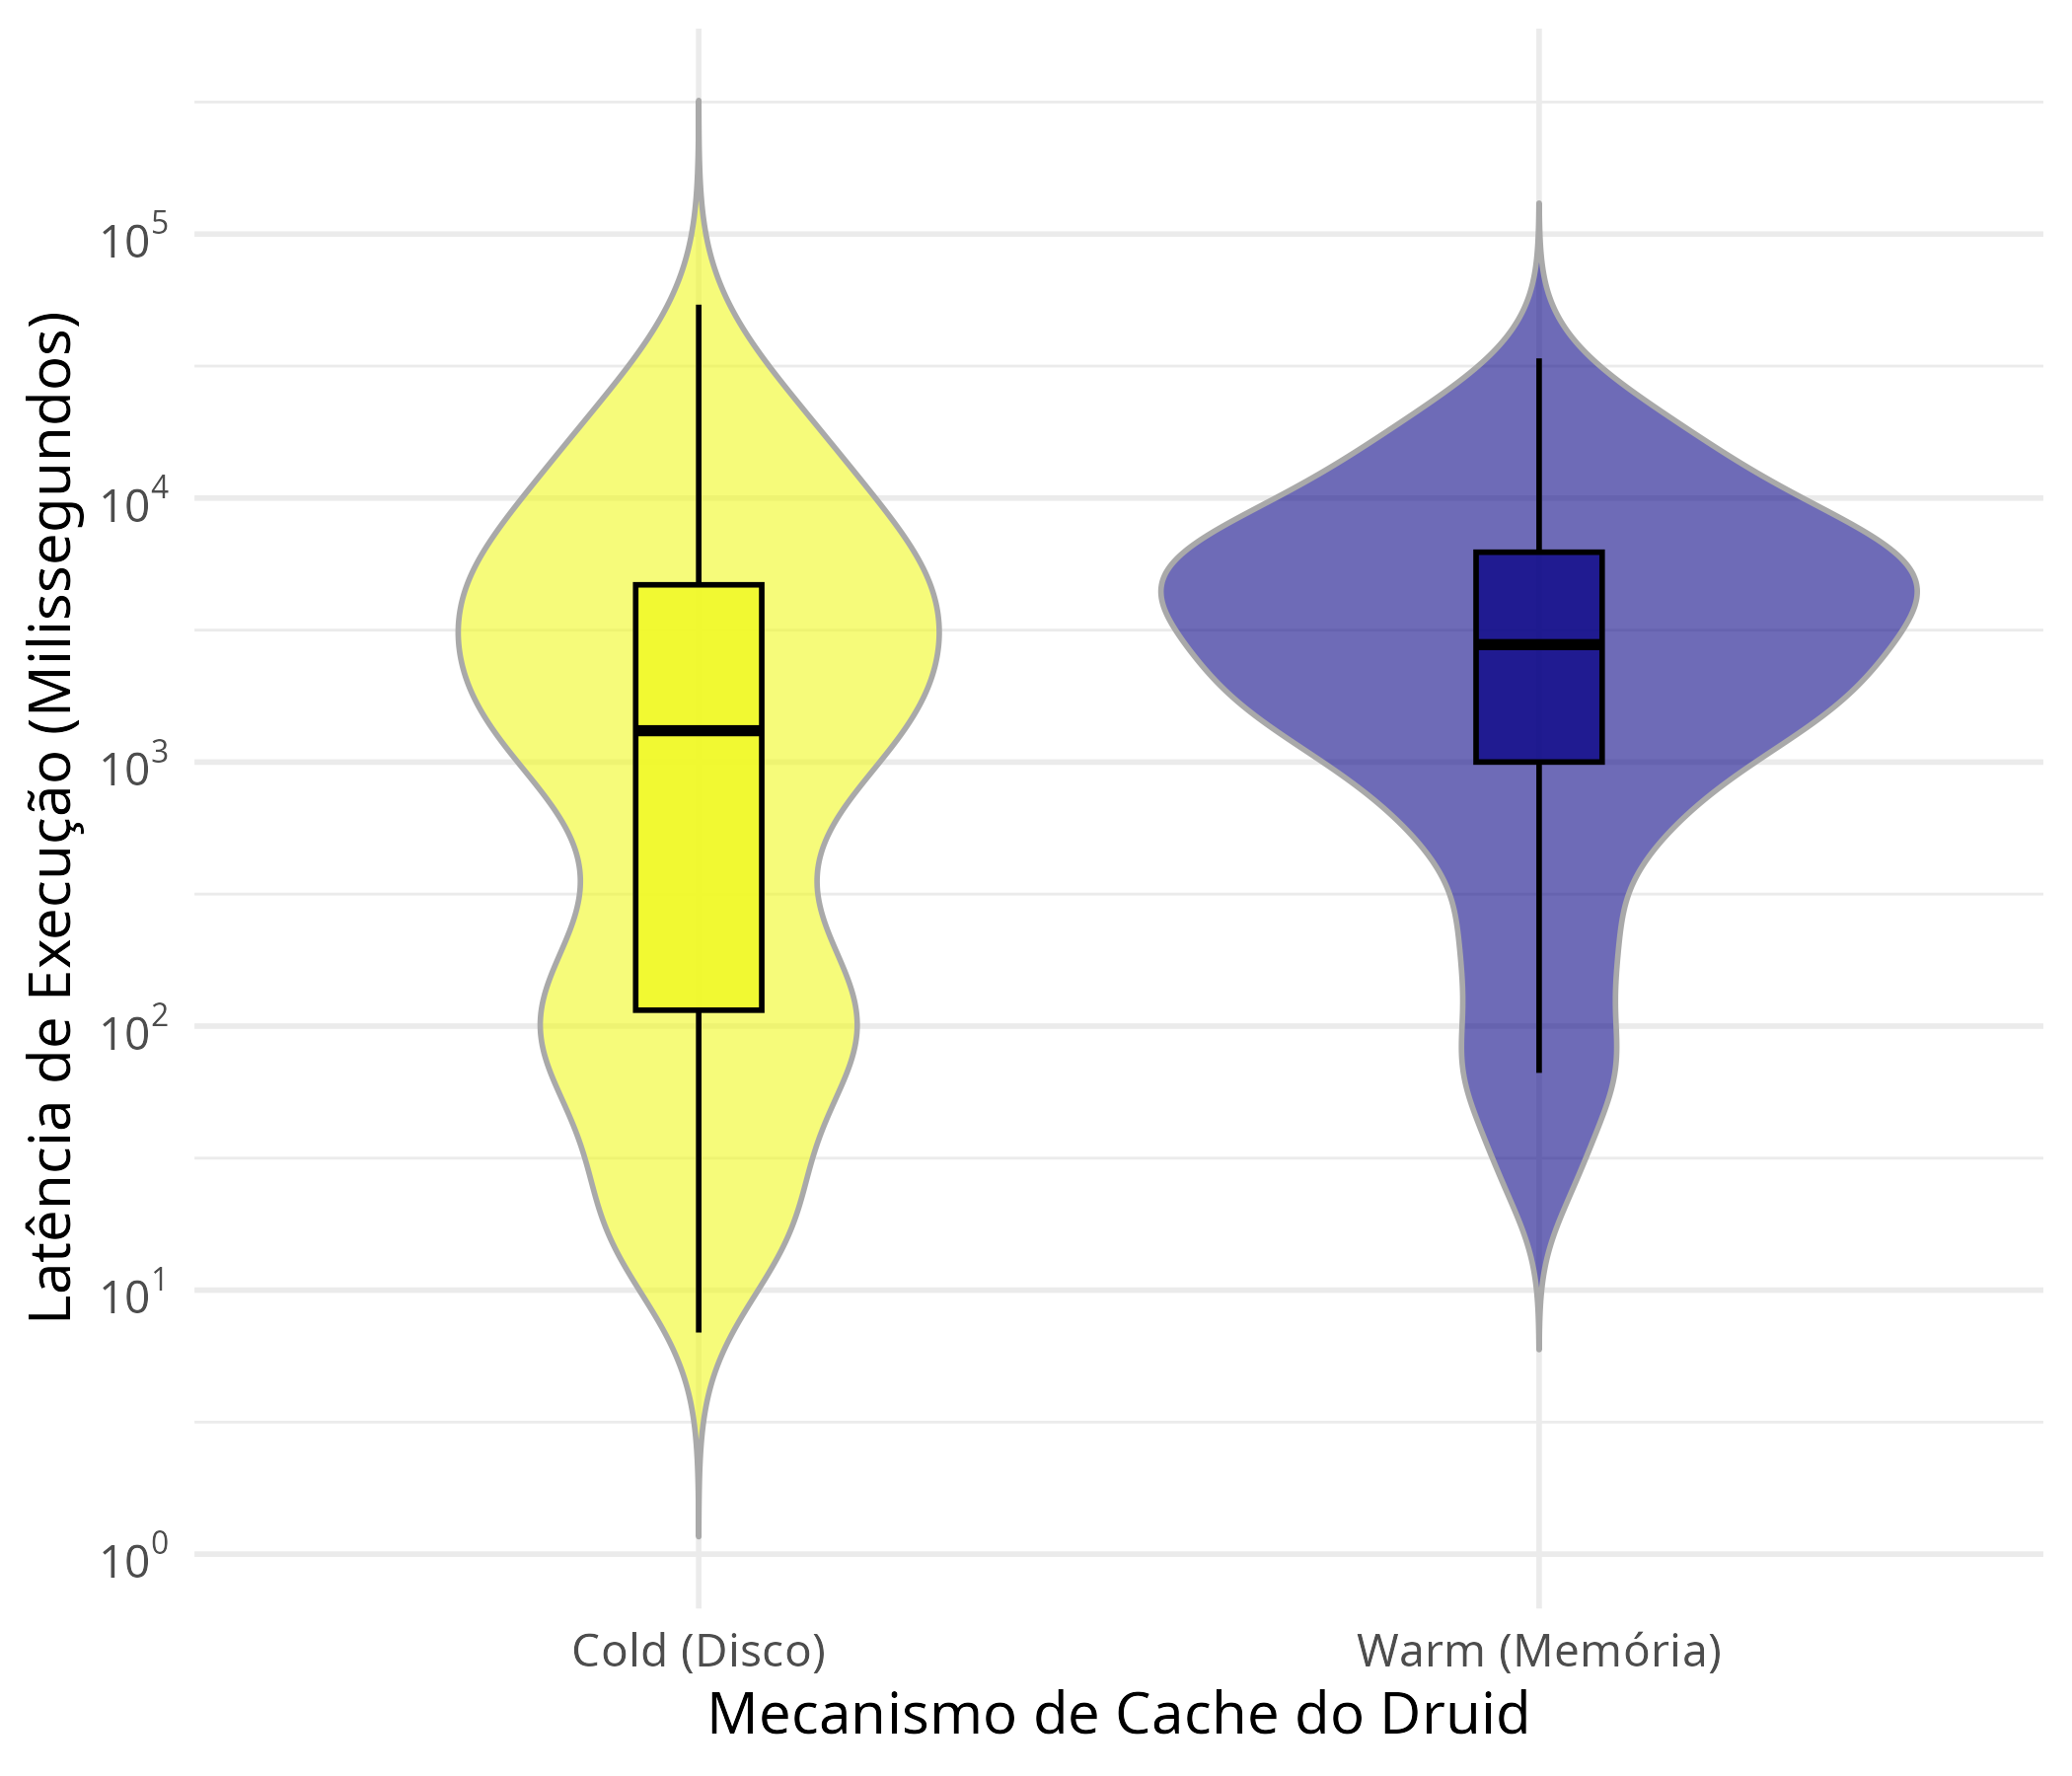
\includegraphics[width=0.8\textwidth]{analise_R/plots/cache_violin_new.png}
    \caption{Distribuição de Latência: Cache vs. Leitura Nativa.}
    \label{fig:cache_efficiency}
\end{figure}

\subsection{Consumo Físico de Contêineres e Esgotamento (Memory Footprint)}

A série temporal corrobora a estabilidade dos nós conteinerizados perante o limite estrito do \textit{Cgroup} (Docker), demonstrando teto rígido (inferior a 90\%) e atestando a ausência de vazamento de memória (\textit{Memory Leak}). O motor de varredura (\textit{Historical}) acomoda-se em platôs seguros (70\%-80\%) durante as rajadas de carga.

De maneira análoga, o contêiner integrador (\textit{Broker}) exibe um comportamento resiliente, evidenciando que grandes cargas cartográficas em memória (GeoJSON) são velozmente serializadas, com espaço recuperado pelas rotinas de limpeza da JVM (\textit{Garbage Collection}). Sem o registro de falhas por esgotamento (\textit{OOM Killed}), conclui-se que o verdadeiro gargalo analítico da plataforma reside no processamento matemático espacial (restrição de vCPU), e não na escassez de RAM.

\begin{figure}[H]
    \centering
    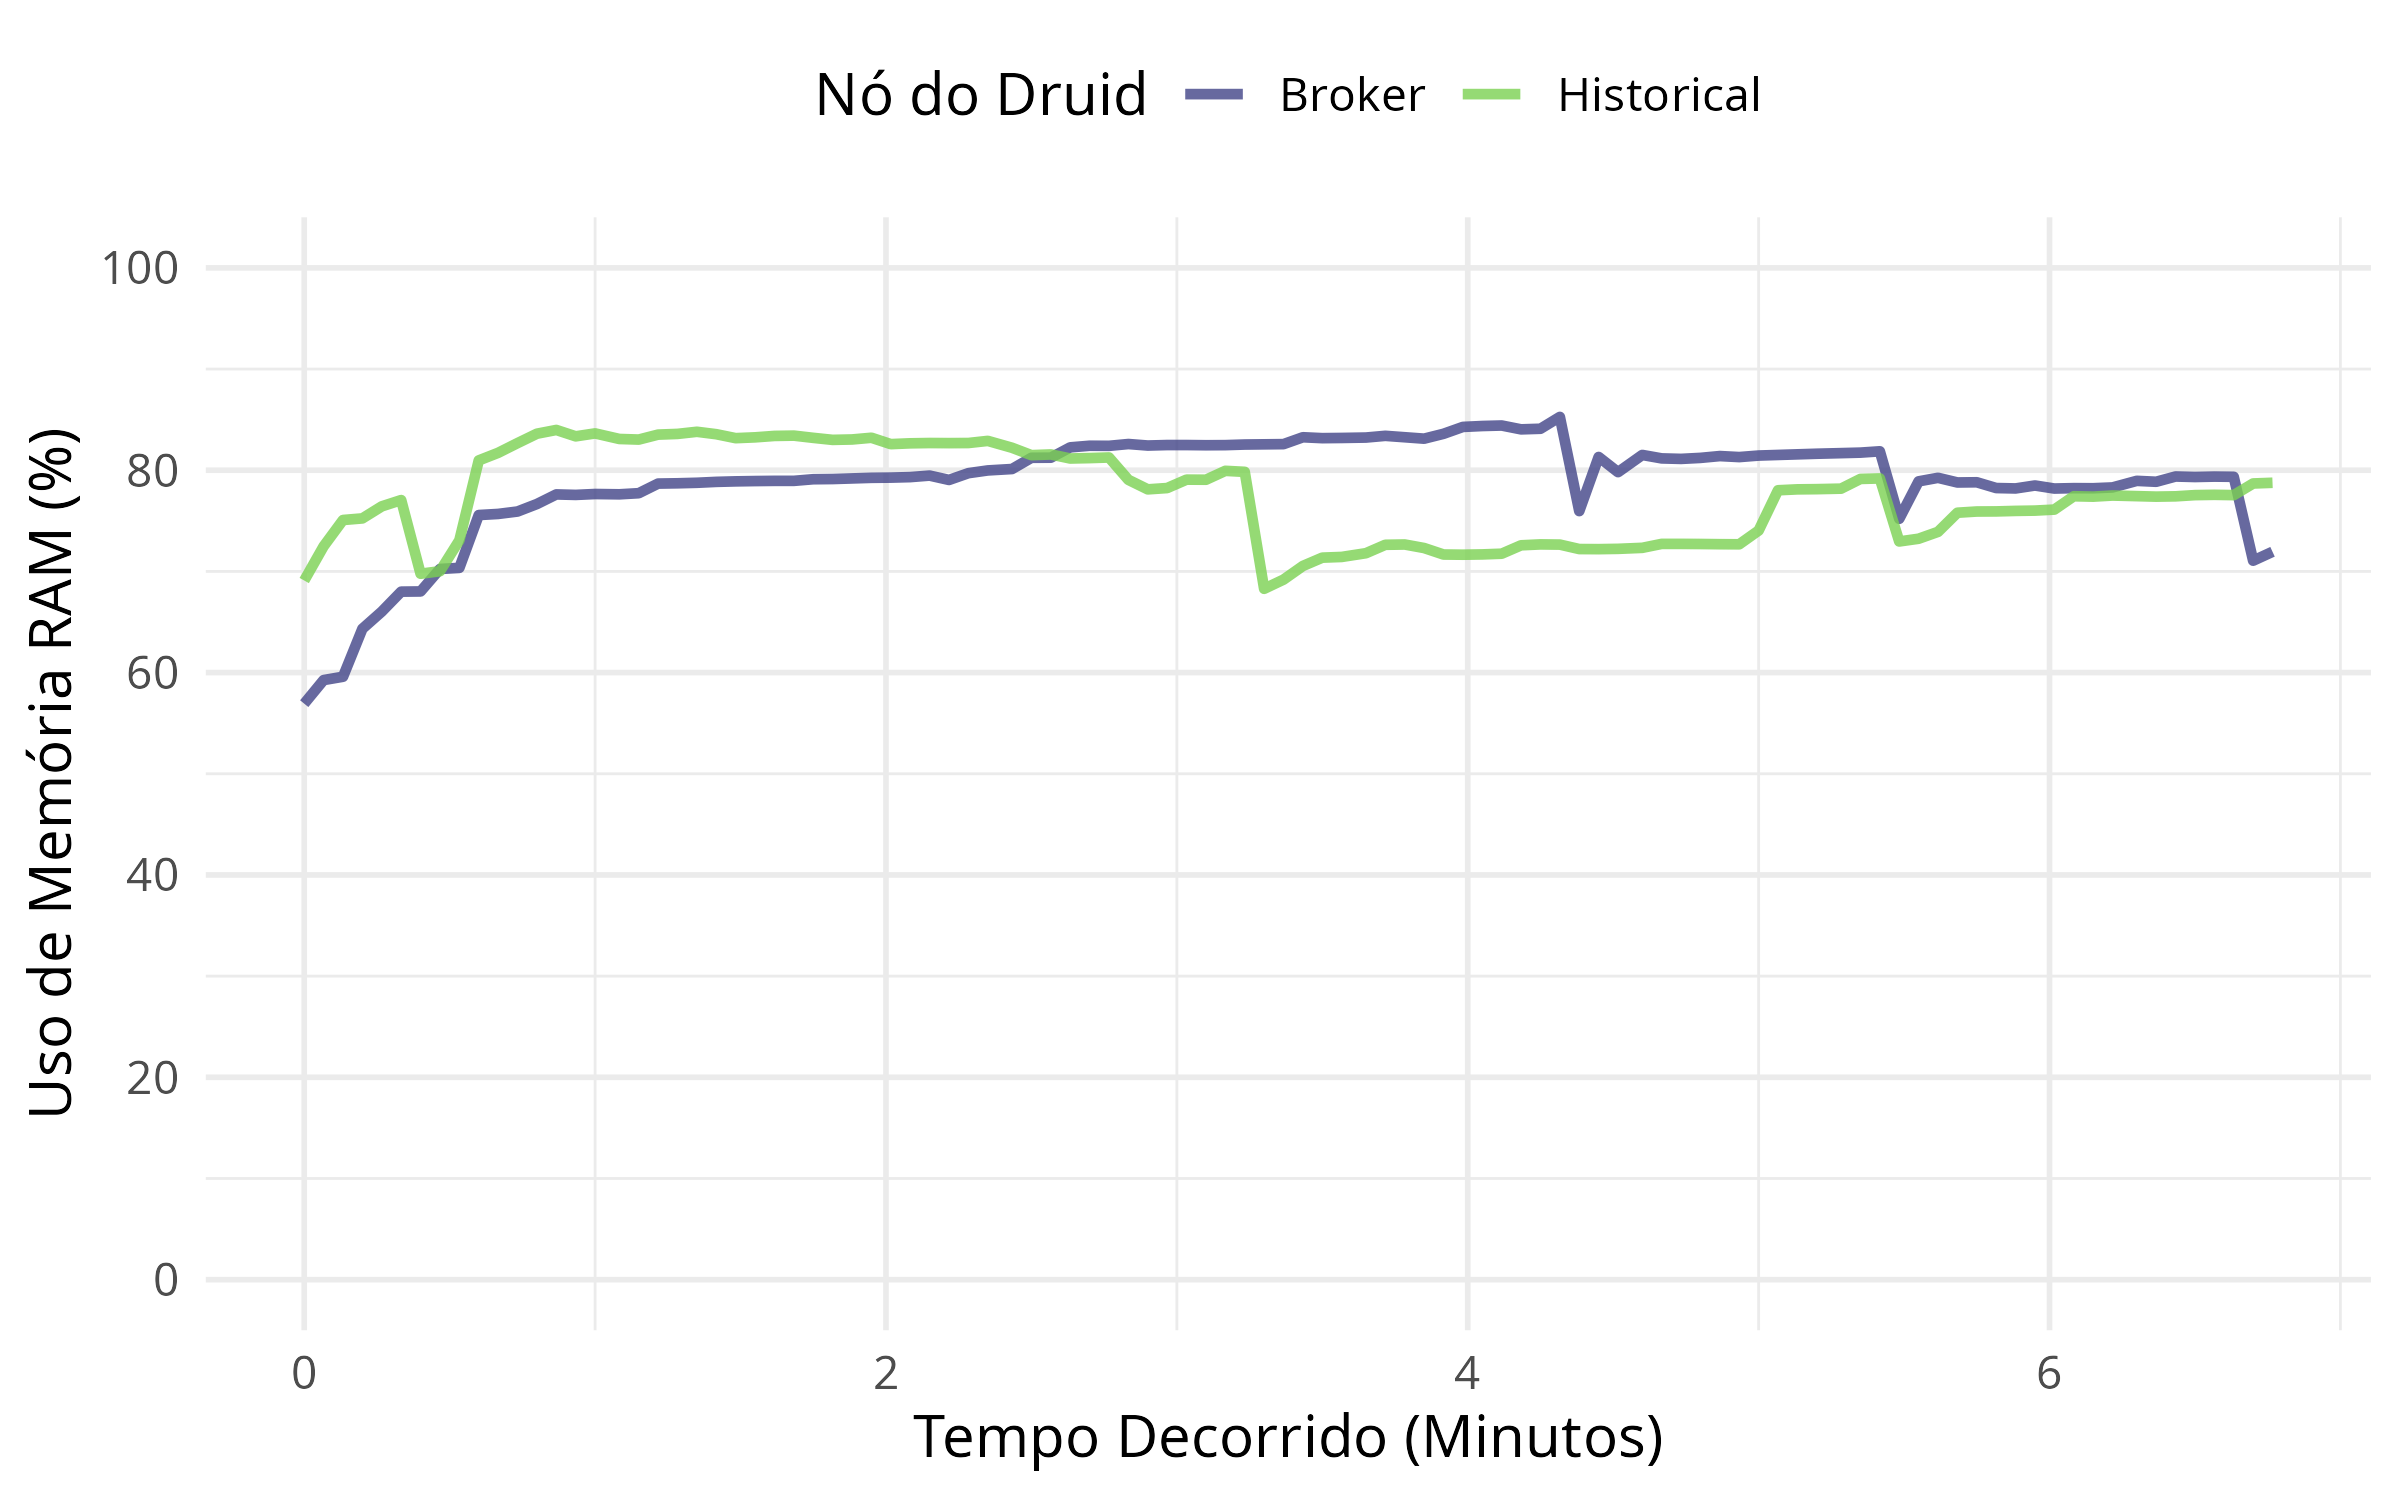
\includegraphics[width=0.8\textwidth]{analise_R/plots/ram_usage_new.png}
    \caption{Oscilação do Consumo de RAM no Apache Druid.}
    \label{fig:ram_usage}
\end{figure}
